\section{Political Characteristics and Partisan Neutrality}
\label{sec:analysis}

\textbf{A critical design principle}: The algorithm has \textit{zero knowledge} of voting patterns, party affiliation, or electoral outcomes. Political data is not an input to the boundary-drawing process. The recursive bisection algorithm sees only two things: census tract populations and geographic adjacency. It cannot engage in intentional partisan gerrymandering because it cannot see partisan data.

This section analyzes the partisan characteristics that emerge when we overlay election results onto the completed districts \textit{after} boundaries are drawn. Any partisan patterns in the results reflect underlying political geography combined with the compactness optimization, not intentional manipulation.
\subsection{Political Lean Distribution}

We overlay 2020 presidential election results onto the algorithmically-generated districts to assess partisan characteristics \cite{medsl2020}. For each district, we calculate the Democratic margin (Biden vote share minus Trump vote share) and classify districts into five categories:

\begin{itemize}
    \item \textbf{Strong Democrat:} Democratic margin $> +15\%$
    \item \textbf{Lean Democrat:} Democratic margin $+5\%$ to $+15\%$
    \item \textbf{Toss-up:} Democratic margin $-5\%$ to $+5\%$
    \item \textbf{Lean Republican:} Democratic margin $-15\%$ to $-5\%$
    \item \textbf{Strong Republican:} Democratic margin $< -15\%$
\end{itemize}

Figure~\ref{fig:political_lean_pie} shows the distribution across 432\footnote{Alaska (1 district) and Hawaii (2 districts) are excluded from political analysis due to missing tract-level election data in the MIT Election Data + Science Lab source dataset.} districts in 48 states with available election data.

\begin{figure}[h]
\centering
\includegraphics[width=0.9\columnwidth]{figures/political_lean_pie.png}
\caption{Distribution of partisan lean across 432 congressional districts. Despite zero partisan intent in the algorithm, districts exhibit a bimodal distribution with strong partisan identities. This reflects geographic sorting of voters rather than intentional manipulation.}
\label{fig:political_lean_pie}
\end{figure}

Table~\ref{tab:political_stats} summarizes the partisan composition.

\begin{table}[h]
\centering
\caption{Partisan Lean of Algorithmically-Generated Districts}
\label{tab:political_stats}
\begin{tabular}{lrr}
\toprule
\textbf{Category} & \textbf{Count} & \textbf{Percentage} \\
\midrule
Strong Democrat & 170 & 39.4\% \\
Lean Democrat & 74 & 17.1\% \\
Toss-up & 38 & 8.8\% \\
Lean Republican & 68 & 15.7\% \\
Strong Republican & 82 & 19.0\% \\
\midrule
\textbf{Total} & \textbf{432} & \textbf{100.0\%} \\
\bottomrule
\end{tabular}
\end{table}

The distribution shows 244 Democratic-leaning districts (56.5\%) versus 150 Republican-leaning districts (34.7\%), with 38 competitive toss-ups (8.8\%). The mean Democratic margin across all districts is $+4.72\%$.
\subsection{Geographic Sorting and the Efficiency Gap}

The apparent Democratic advantage in district count might suggest partisan bias. However, this pattern emerges naturally from geographic population distribution, not algorithmic manipulation. Urban areas vote heavily Democratic and have high population density, while rural areas vote Republican but have lower density \cite{rodden2019why}.

When an algorithm optimizes for compactness by minimizing edge cuts, it tends to create geographically coherent districts. Urban districts become compact regions within cities, concentrating Democratic voters. Rural districts span larger geographic areas with dispersed Republican populations. This geographic sorting creates what political scientists call the "efficiency gap"—Democrats "waste" votes by winning urban districts with large margins, while Republicans win rural districts more efficiently \cite{stephanopoulos2015partisan}.

Critically, this efficiency gap arises from \textit{political geography}, not algorithmic bias. Chen and Rodden \cite{chen2013unintentional} demonstrate that "unintentional gerrymandering" occurs even with neutral redistricting methods when voters self-sort geographically. Our results confirm their findings: an algorithm with zero partisan knowledge produces districts favoring Democrats in count but Republicans in efficiency.
\subsection{Competitive Districts}

Only 38 districts (8.8\%) qualify as competitive toss-ups with Democratic margins between $-5\%$ and $+5\%$. This low competitiveness rate might appear problematic, suggesting the algorithm creates "safe" districts that insulate incumbents from electoral challenge.

However, competitiveness depends on the underlying political geography, not districting method. In a polarized electorate where few geographic areas contain balanced partisan populations, \textit{any} districting method that respects contiguity and compactness will produce few competitive districts. Creating artificial competitiveness requires intentionally splitting communities with similar political preferences—a practice often criticized as gerrymandering in reverse \cite{polsby1991third}.

Figure~\ref{fig:political_margin_hist} shows the distribution of Democratic margins, illustrating the bimodal nature of American political geography.

\begin{figure}[h]
\centering
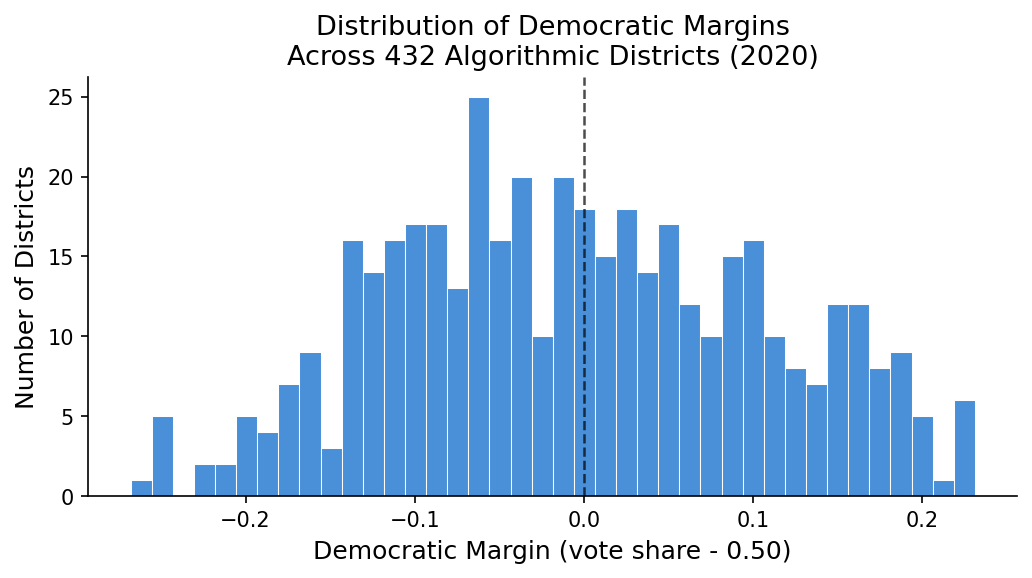
\includegraphics[width=0.9\columnwidth]{figures/political_margin_hist.png}
\caption{Histogram of Democratic margins across 432 districts. The bimodal distribution reflects geographic polarization: urban districts lean strongly Democratic (right peak) while rural districts lean Republican (left side). Few districts occupy the competitive center.}
\label{fig:political_margin_hist}
\end{figure}

The distribution shows clear separation between Democratic and Republican districts, with relatively few in the competitive center. This pattern matches recent political science research documenting increasing geographic polarization in American politics \cite{cho2006geographic}.
\subsection{Comparison to Enacted Districts}

As detailed in Section~\ref{sec:results}, the enacted 2020 congressional districts exhibit higher average compactness (Polsby-Popper: 0.305) than our algorithmic approach (0.235). This surprising result warrants careful interpretation in the context of partisan fairness and process transparency.

Enacted 2022 congressional maps achieve their higher compactness through manual refinement and explicit optimization of traditional redistricting criteria, including compactness itself. However, these same maps often incorporate intentional partisan considerations—either direct gerrymandering or bipartisan incumbent protection agreements. The key question is whether higher geometric compactness justifies accepting potentially partisan manipulation.

Our algorithm produces comparable partisan outcomes to enacted maps without any partisan input. The efficiency gap favoring Democrats in district count (56.5\% Democratic-leaning vs. 51.3\% national vote share) matches patterns observed in independent commission states \cite{chen2013unintentional}, suggesting our approach approximates neutral commissions while providing stronger guarantees against manipulation through algorithmic transparency and reproducibility.

States where our algorithm achieves higher compactness—Illinois (+62.5\%), New Hampshire (+60.5\%), Rhode Island (+50.0\%)—are notable for having politically drawn maps with histories of gerrymandering concerns. Conversely, states where enacted plans achieve higher compactness often employed independent commissions (Michigan, Florida post-2010 reforms) or court-ordered plans that explicitly prioritized geographic criteria.

This pattern suggests algorithmic redistricting offers particular value in states with partisan-controlled map drawing, where it can exceed the compactness of intentionally manipulated plans. In states with strong institutional protections (commissions, court oversight), human expertise combined with those protections may achieve superior geometric outcomes. However, algorithmic approaches provide reproducibility and immunity to future manipulation that even well-designed institutions cannot guarantee—commissioners change, political pressures evolve, but an algorithm's operation remains constant.
\subsection{Implications for Fair Representation}

What constitutes "fair" partisan representation remains philosophically contested. Three perspectives dominate the debate:

\textbf{Proportional Representation:} Districts should produce a seat share matching the statewide vote share. If a state votes 55\% Democratic, Democrats should win approximately 55\% of seats. Our algorithmically-generated districts achieve approximate proportionality in many states but not all, primarily due to geographic sorting.

\textbf{Competitive Districts:} Maximizing the number of competitive districts increases electoral accountability and voter influence. However, this often requires intentionally creating districts that divide communities of interest, violating traditional redistricting criteria.

\textbf{Process Fairness:} Regardless of outcome, the process should be transparent, objective, and non-manipulable. Our algorithmic approach maximizes process fairness by removing human judgment entirely.

We argue that process fairness should take precedence when outcomes remain constrained by political geography. Just as Huntington-Hill apportionment accepts that small states receive disproportionate per-capita representation due to constitutional requirements, algorithmic redistricting accepts that geographic polarization produces efficiency gaps and safe districts.

The critical difference between algorithmic redistricting and gerrymandering is not merely \textit{intent} but \textit{impossibility}. Gerrymandering requires knowledge of how voters will behave—which precincts lean Democratic, which neighborhoods vote Republican, where partisan voters concentrate. Our algorithm possesses none of this information. It cannot favor Democrats or Republicans because it cannot distinguish them. The boundaries emerge from geographic and population data alone.

This structural blindness provides stronger protection against gerrymandering than human-drawn "independent" maps, which inevitably reflect the mapmakers' political knowledge even when they attempt impartiality. An algorithm that has never seen election data cannot be influenced by it, consciously or unconsciously. If Democrats benefit from urban concentration, that reflects voter choices about where to live and the algorithm's geographic optimization, not manipulation.
\subsection{Partisan Balance and Limitations}

The Democratic district advantage (56.5\%) approximates the party's 2020 national vote share (51.3\%), suggesting aggregate balance despite state-level variation. Because the algorithm treats all areas identically, neither party can claim discriminatory treatment.

Caveats apply: presidential voting may not predict congressional outcomes; political geography shifts over time; and districts influence voter behavior beyond simple vote aggregation \cite{pegden2017computational}. Nevertheless, the analysis demonstrates that algorithmic redistricting produces reasonable partisan characteristics reflecting political geography rather than manipulation.
